\documentclass{IEEEcsmag}

\usepackage[colorlinks,urlcolor=blue,linkcolor=blue,citecolor=blue]{hyperref}

\usepackage{upmath}

\jvol{XX}
\jnum{XX}
\paper{X}
\jmonth{May}
\jname{Computing in Science and Engineering}
\pubyear{2023}
\newtheorem{theorem}{Theorem}
\newtheorem{lemma}{Lemma}
\setcounter{secnumdepth}{0}

\begin{document}

\sptitle{Department: Head}
\editor{Editor: Name, xxxx@email}

\title{Statistical Generation of Ocean Forcing with Realistic Spatiotemporal Variability for Ice Sheet Models}

\author{S. Muruganandham}
\affil{Georgia Institute of Technology}
\author{A.A. Robel}
\affil{Georgia Institute of Technology}
\author{M. Hoffman}
\affil{Los Alamos National Laboratory}
\author{S. Price}
\affil{Los Alamos National Laboratory}
\markboth{Department Head}{Paper title}

\begin{abstract}
Basal melting of floating ice shelves fringing the Antarctic Ice Sheet (AIS) has been identified as a significant driver of uncertainty in sea level rise (SLR) projections. Part of this uncertainty derives from unpredictable internal variability in oceanic and atmospheric temperatures around ice shelves, in addition to poorly understood glaciological processes. However, quantifying this uncertainty with ensembles of climate and ice model simulations is prohibitively computationally expensive. Here, we develop and demonstrate a statistical technique that generates random realisations of basal melt rate projections which emulate a single long simulation from the Energy Exascale Earth System Model (E3SM) in a computationally efficient manner. This generation technique ensures spatially and temporally consistent variability, while also facilitating the sampling of a wide range of melt trajectories. Each such ensemble member can be characterised as an independent realisation of the ice sheet model simulation output with variable thermal forcing.
\end{abstract}
\maketitle
%\section{INTRODUCTION}
\chapterinitial{Basal melting} of ice shelves in marine ice sheets (the Antarctic Ice Sheet?) is a control for the stability of the ice sheet and global sea level rise projections. It has been identified as a significant driver of uncertainty in sea-level rise (SLR) projections.A part of this uncertainty derives from unpredictable internal variability in ocean and atmosphere temperatures around ice shelves. This uncertainty can be quantified using large ensembles of ice sheet model simulations, with each ensemble member influenced by an alternate realization of such external climate variable evolution (climate "forcing"). However, running such a large number of climate and ice sheet simulations is computationally prohibitive. Here, we develop and demonstrate a statistical technique that generates random realisations of basal melt rate projections which emulate a single long simulation from the Energy Exascale Earth System Model (E3SM) in a computationally efficient manner. Internal climate variability plays an important role in influencing  basal melt of ice shelves, which in turn can affect the stability of the ice sheet and global sea level rise.
\section{METHOD}
In this study, we use a statistical approach to generate realistic ocean forcing with spatiotemporal variability for ice sheet models. This generation technique ensures spatially and temporally consistent variability, while also facilitating the sampling of a wide range of melt trajectories. We first use a high resolution earth system model to simulate the ocean driven meltwater flux around the southern ocean, i.e., the ocean forcing. Empirical Orthogonal Function (EOF) decomposition is used to emulate spatial variability fields, given that EOFs retain spatial correlation properties across the domain.The projection coefficients from the EOF analysis are then phase randomised to emulate temporal variability fields and generate reconstructed ensemble realisations of the basal melt trajectories.Each such ensemble member can be characterised as an independent realisation of the ice sheet model simulation output with variable thermal forcing.

\subsection{Pre-processing}
\subsection{Spatial Decomposition}
\subsection{Temporal Decomposition}
\subsection{Statistical Generation}

EOF and Fourier phase randomization - explain. Reference fldgen.


\section{RESULTS}
\subsection{Data Description}

\subsection{...}
We evaluate the statistical properties of the resulting ocean forcing realizations by comparing it to the original simulation. We find that the forcing is realistic and that it captures the relevant spatial and temporal variability.

\begin{figure}
\centerline{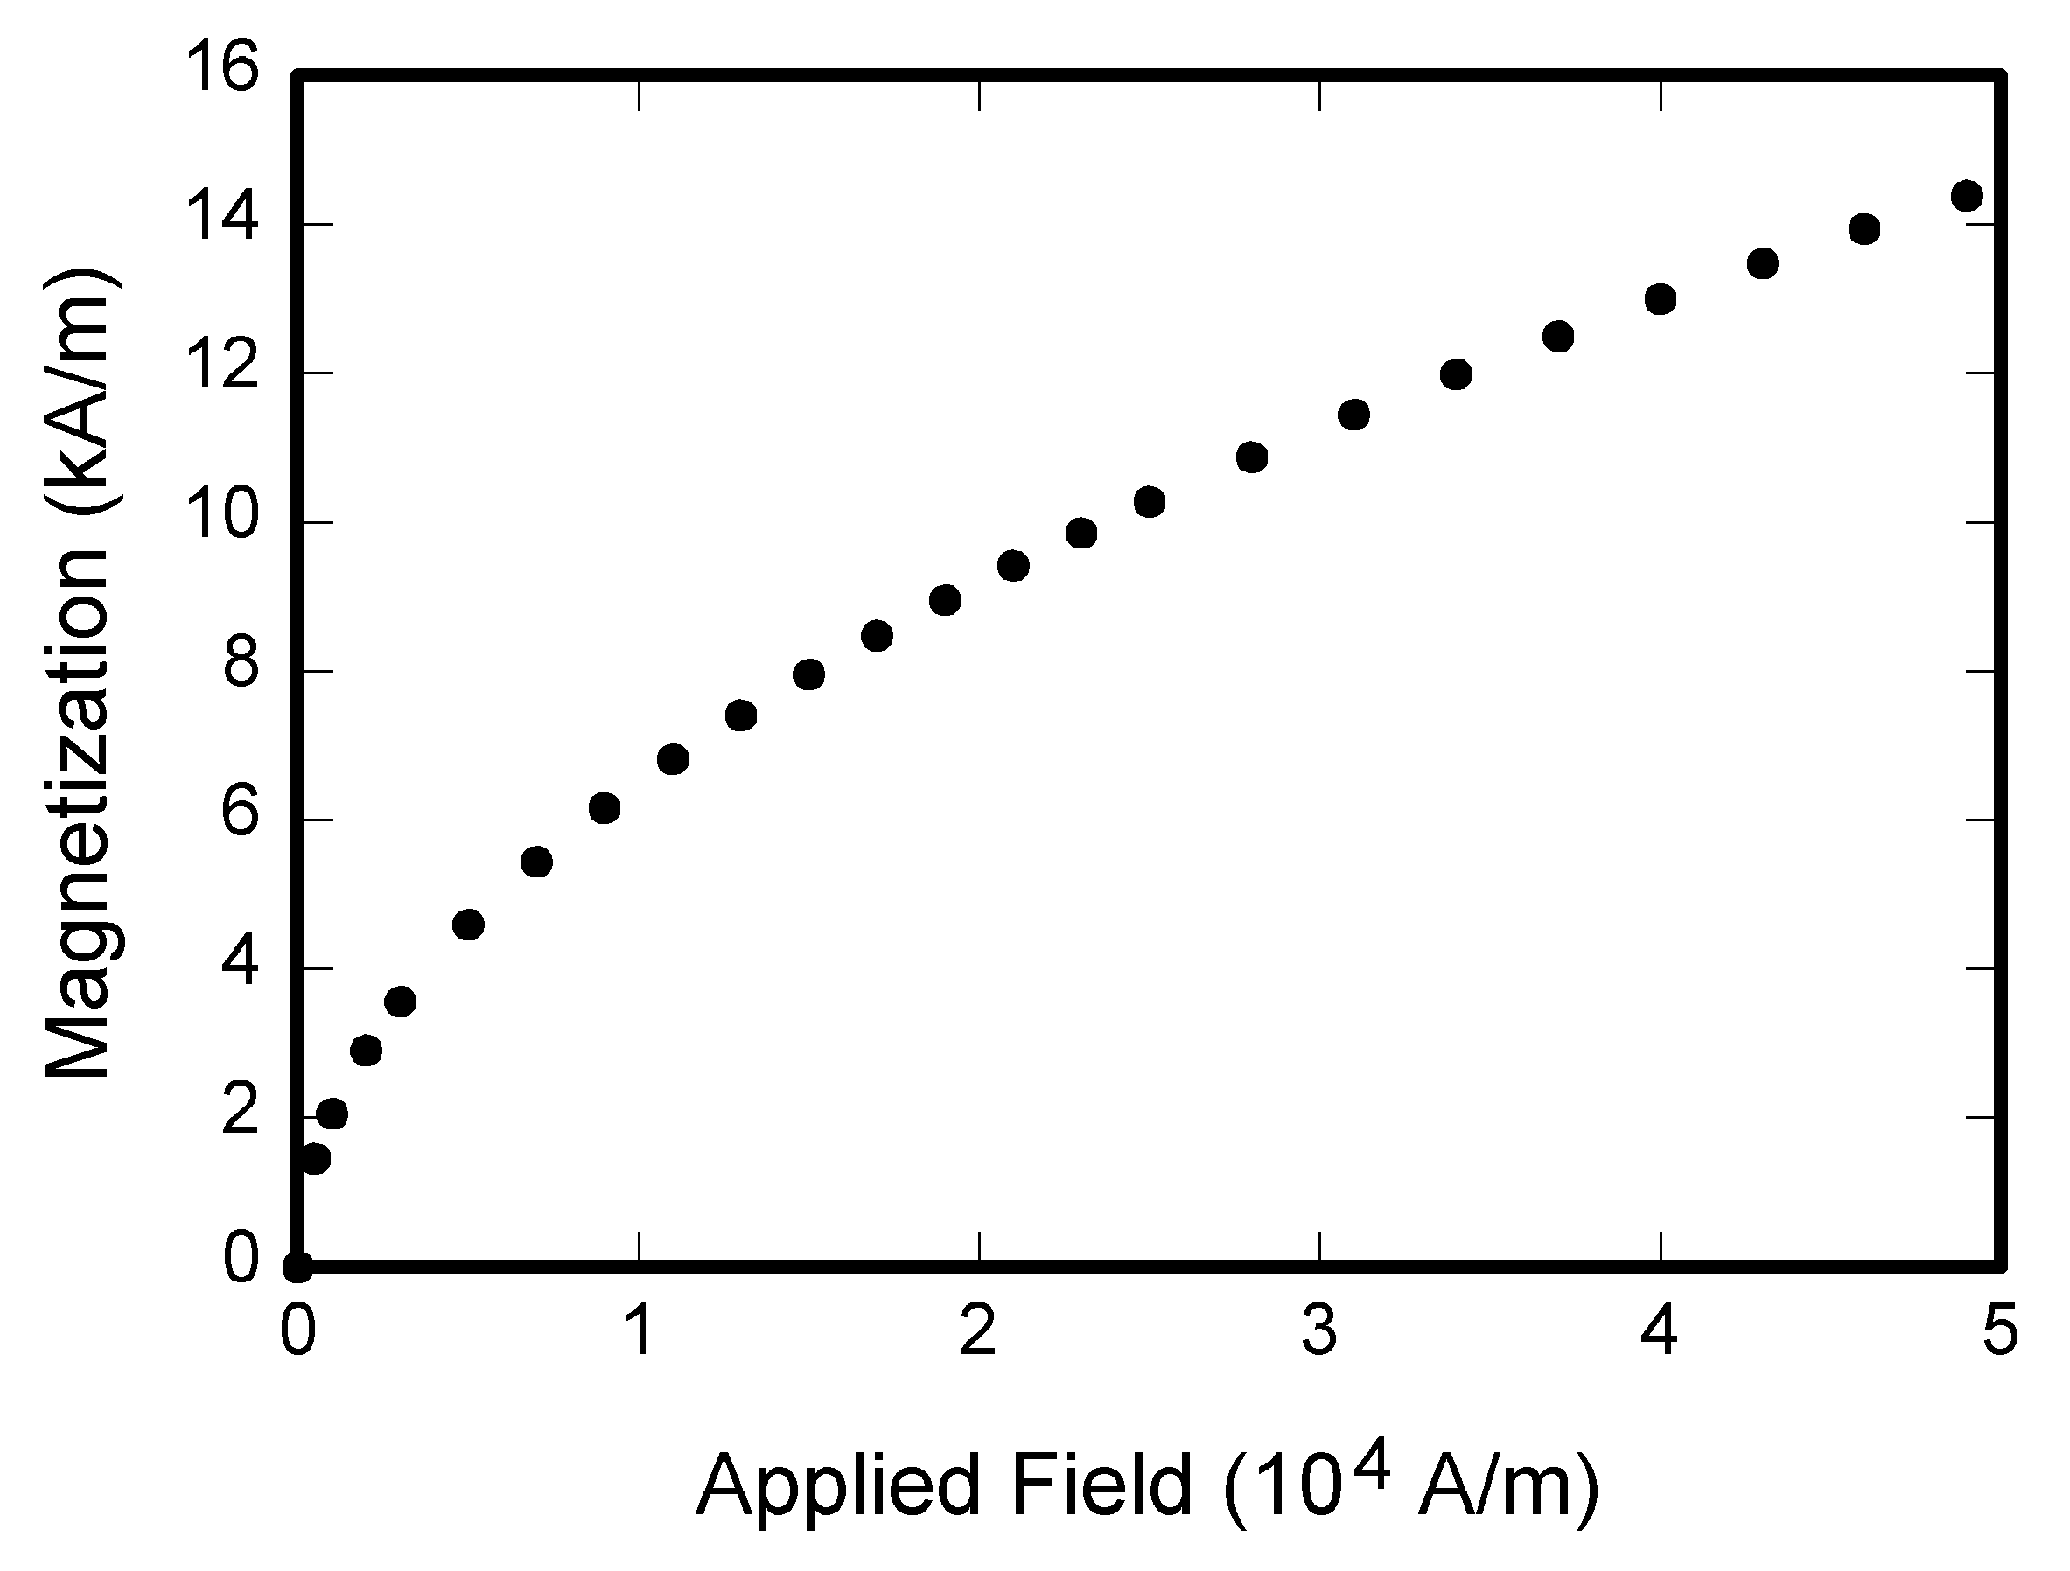
\includegraphics[width=18.5pc]{fig/fig1.png}}
\caption{Workflow / schematic of the generator}
\end{figure}

\begin{figure}
\centerline{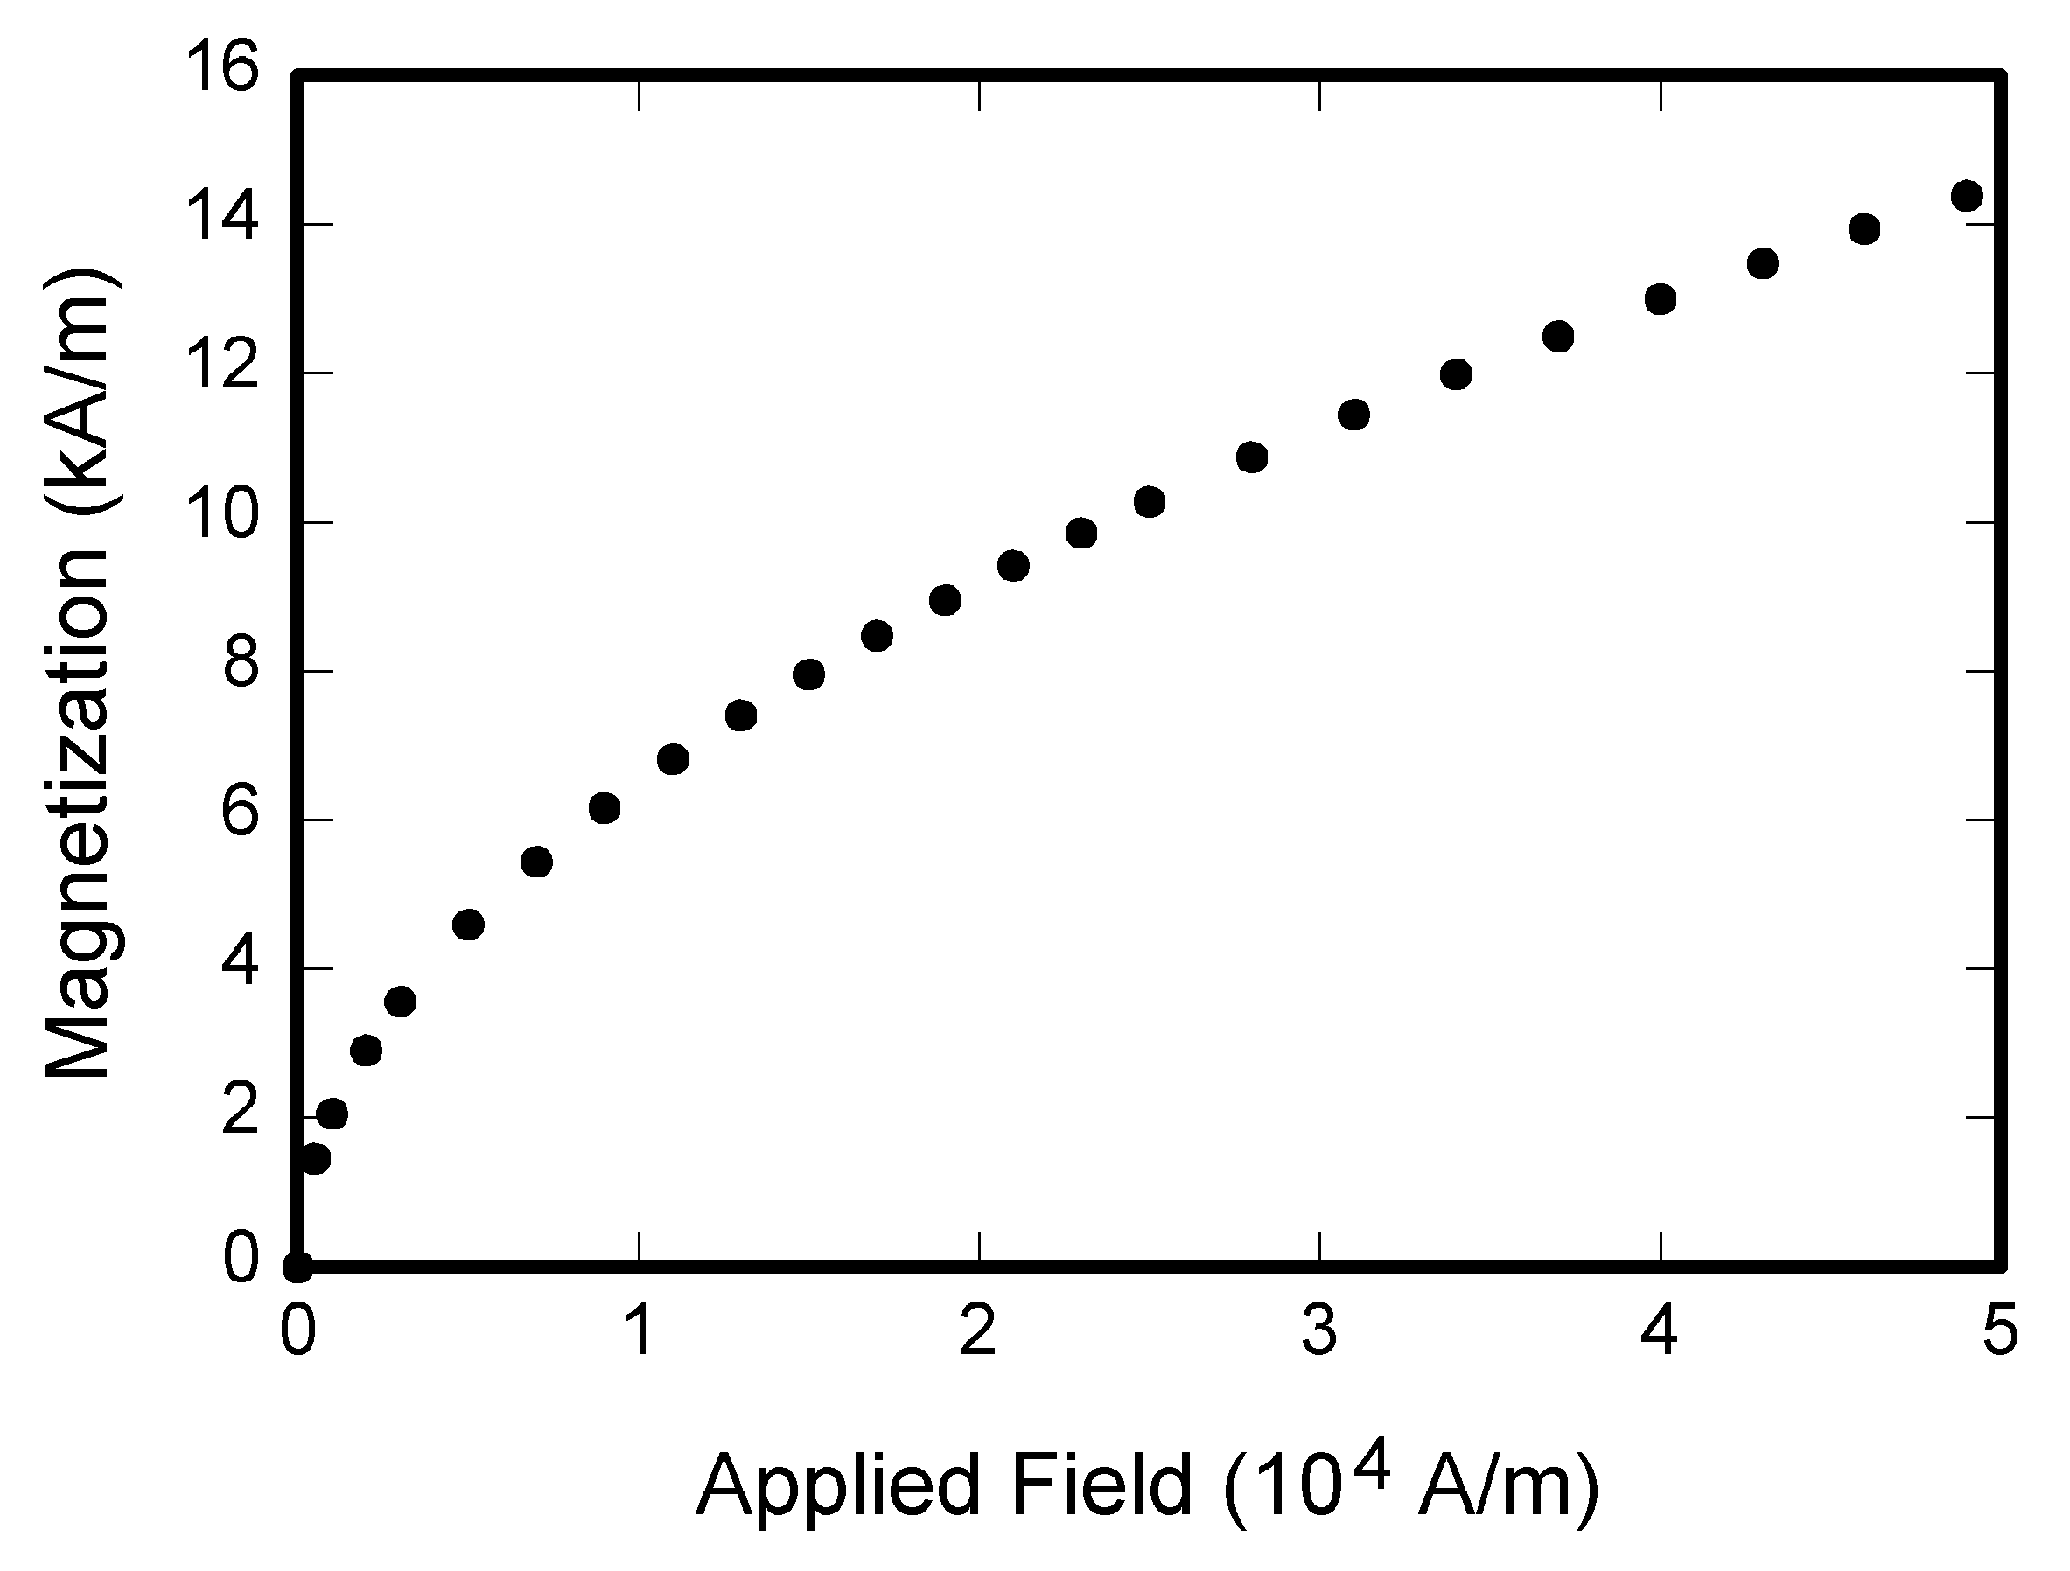
\includegraphics[width=18.5pc]{fig/fig1.png}}
\caption{Map of Antarctic basins used for dedrafting}
\end{figure}

\begin{figure}
\centerline{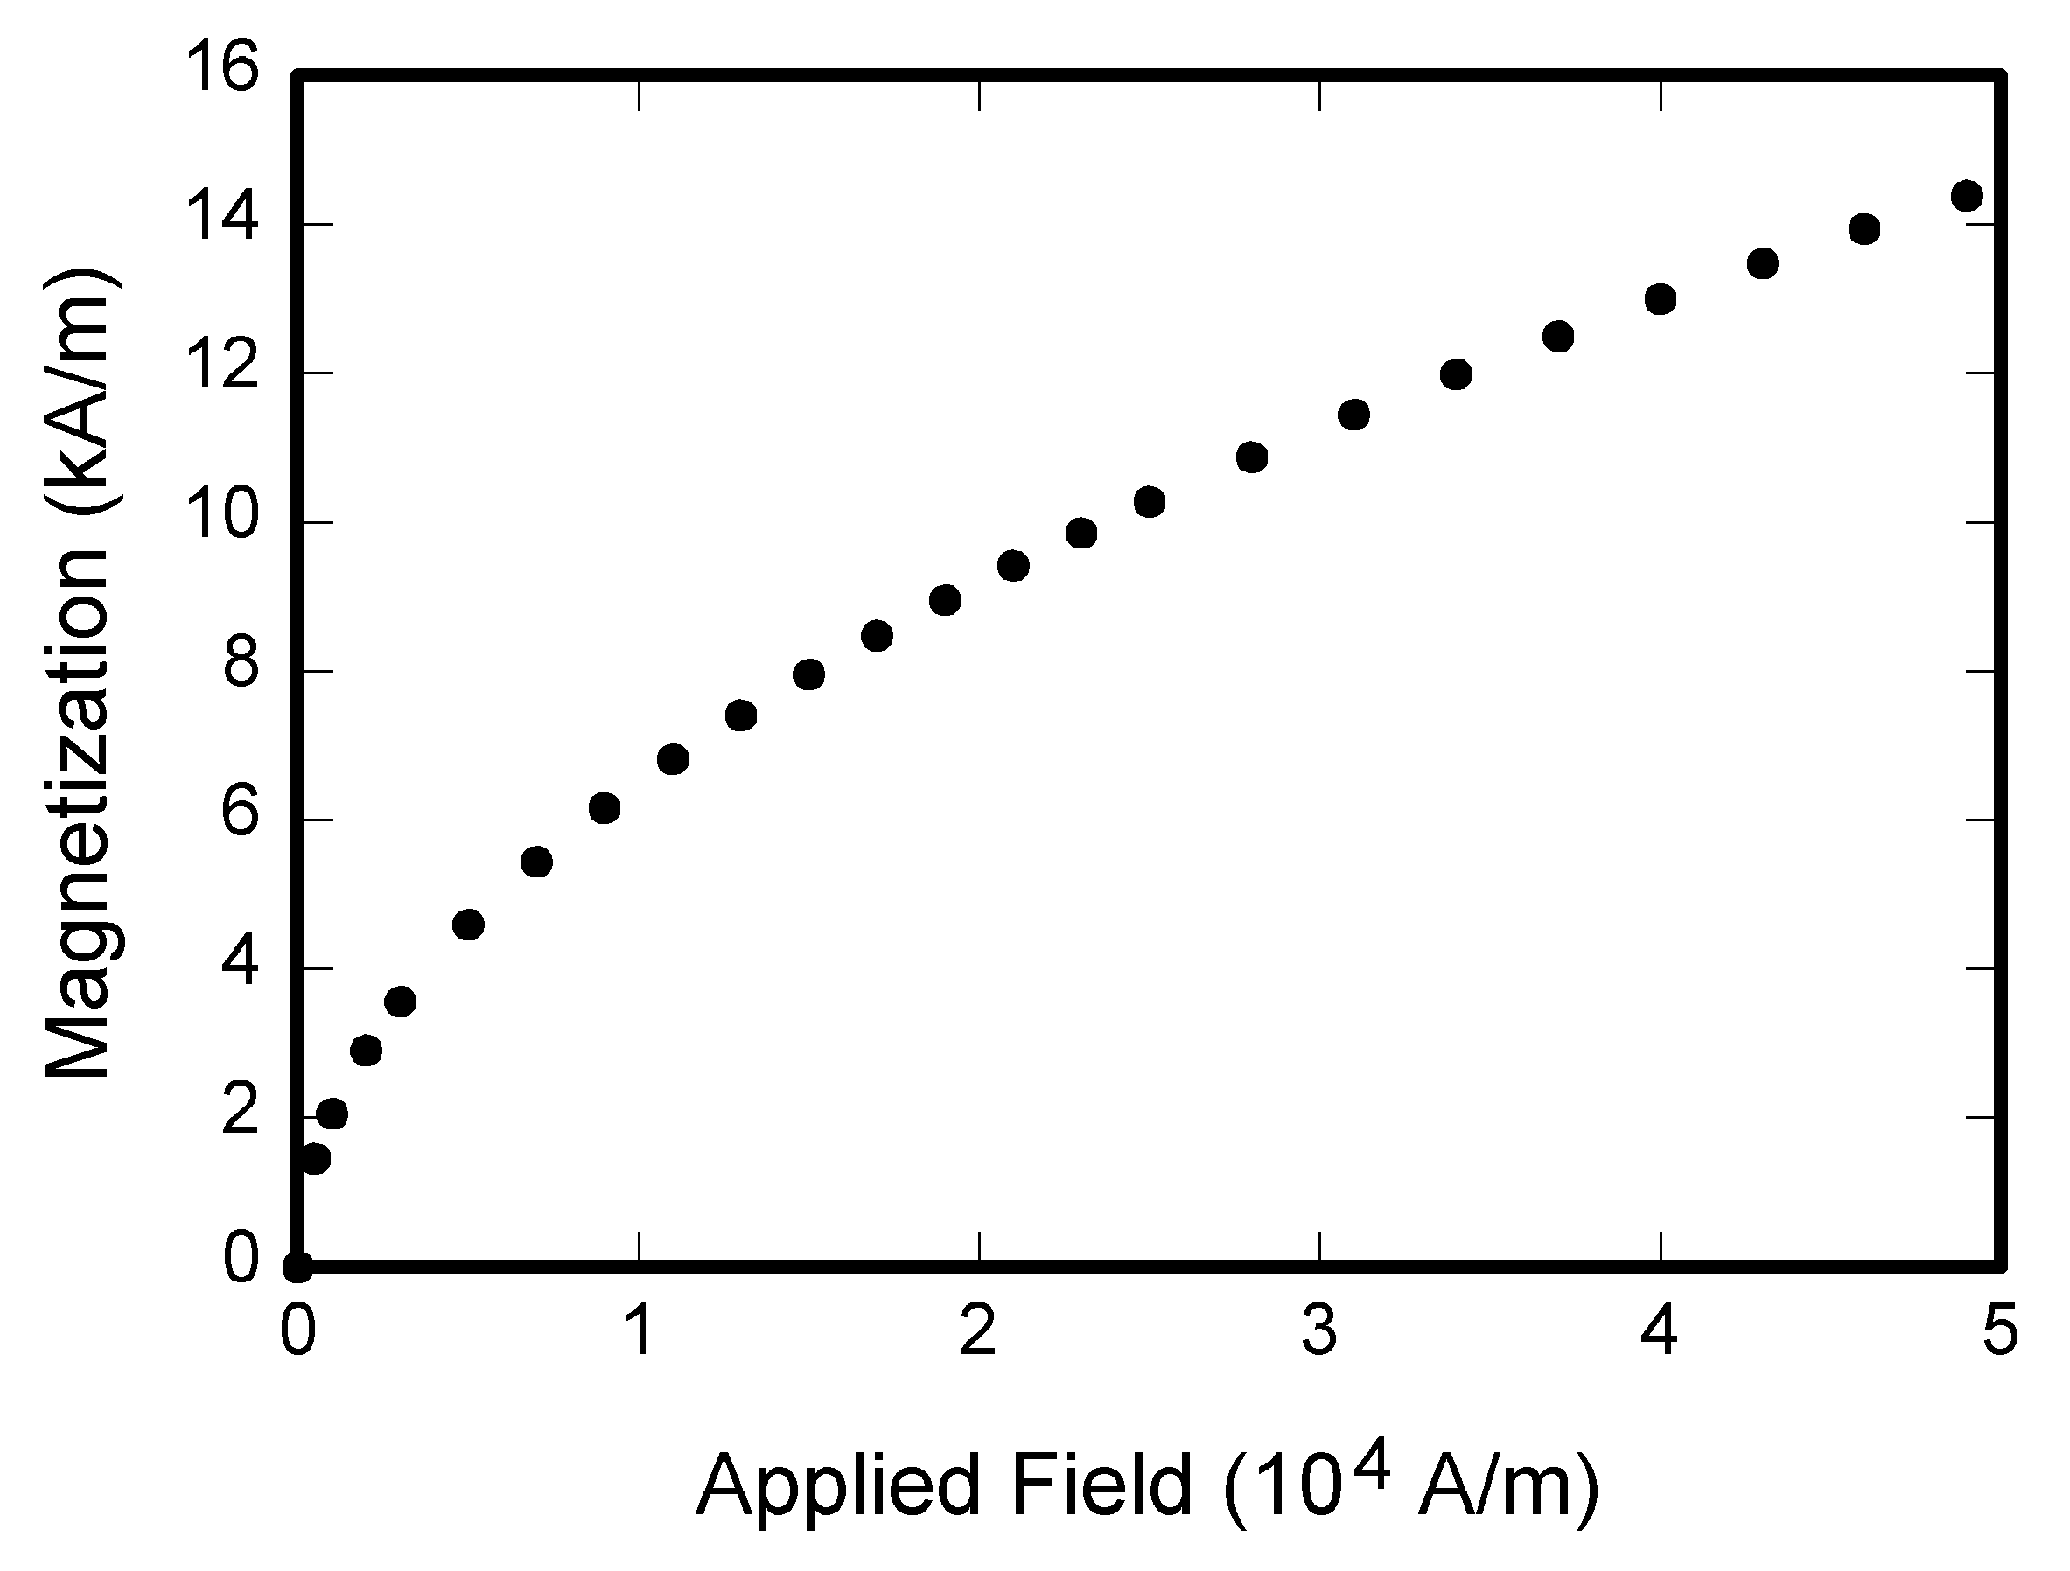
\includegraphics[width=18.5pc]{fig/fig1.png}}
\caption{Melt-draft relationship for different ice shelves, seasonality - can this be an inset?}
\end{figure}

\begin{figure}
\centerline{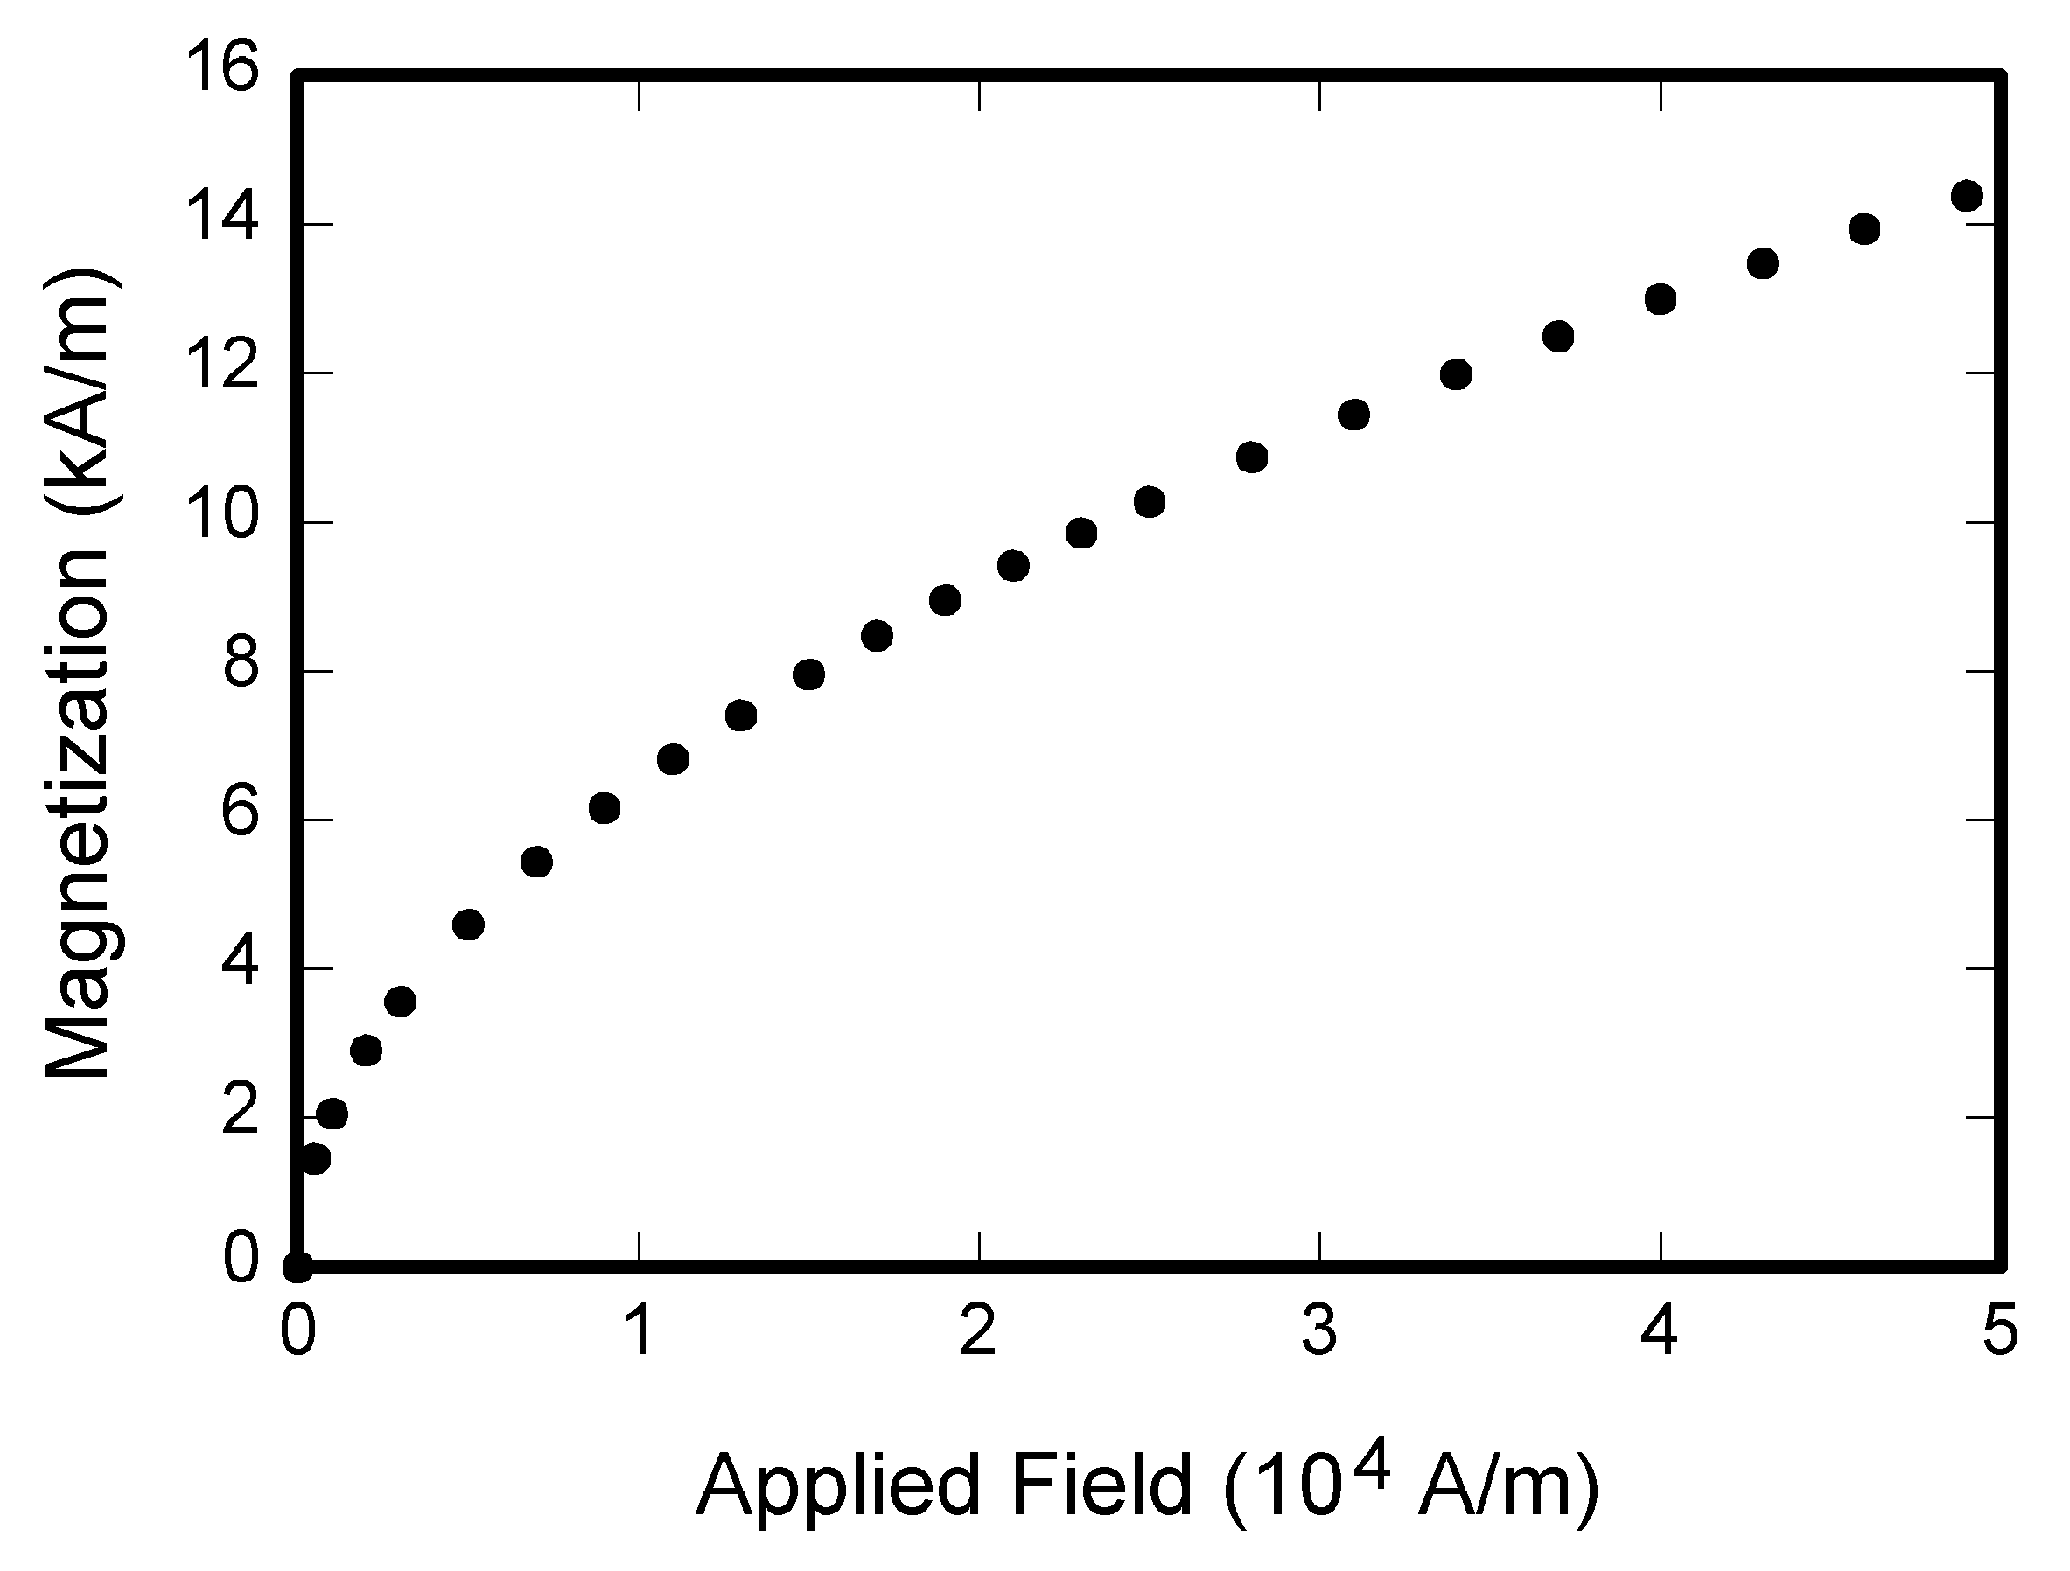
\includegraphics[width=18.5pc]{fig/fig1.png}}
\caption{correlation analyses within and across ice shelves}
\end{figure}

\begin{figure}
\centerline{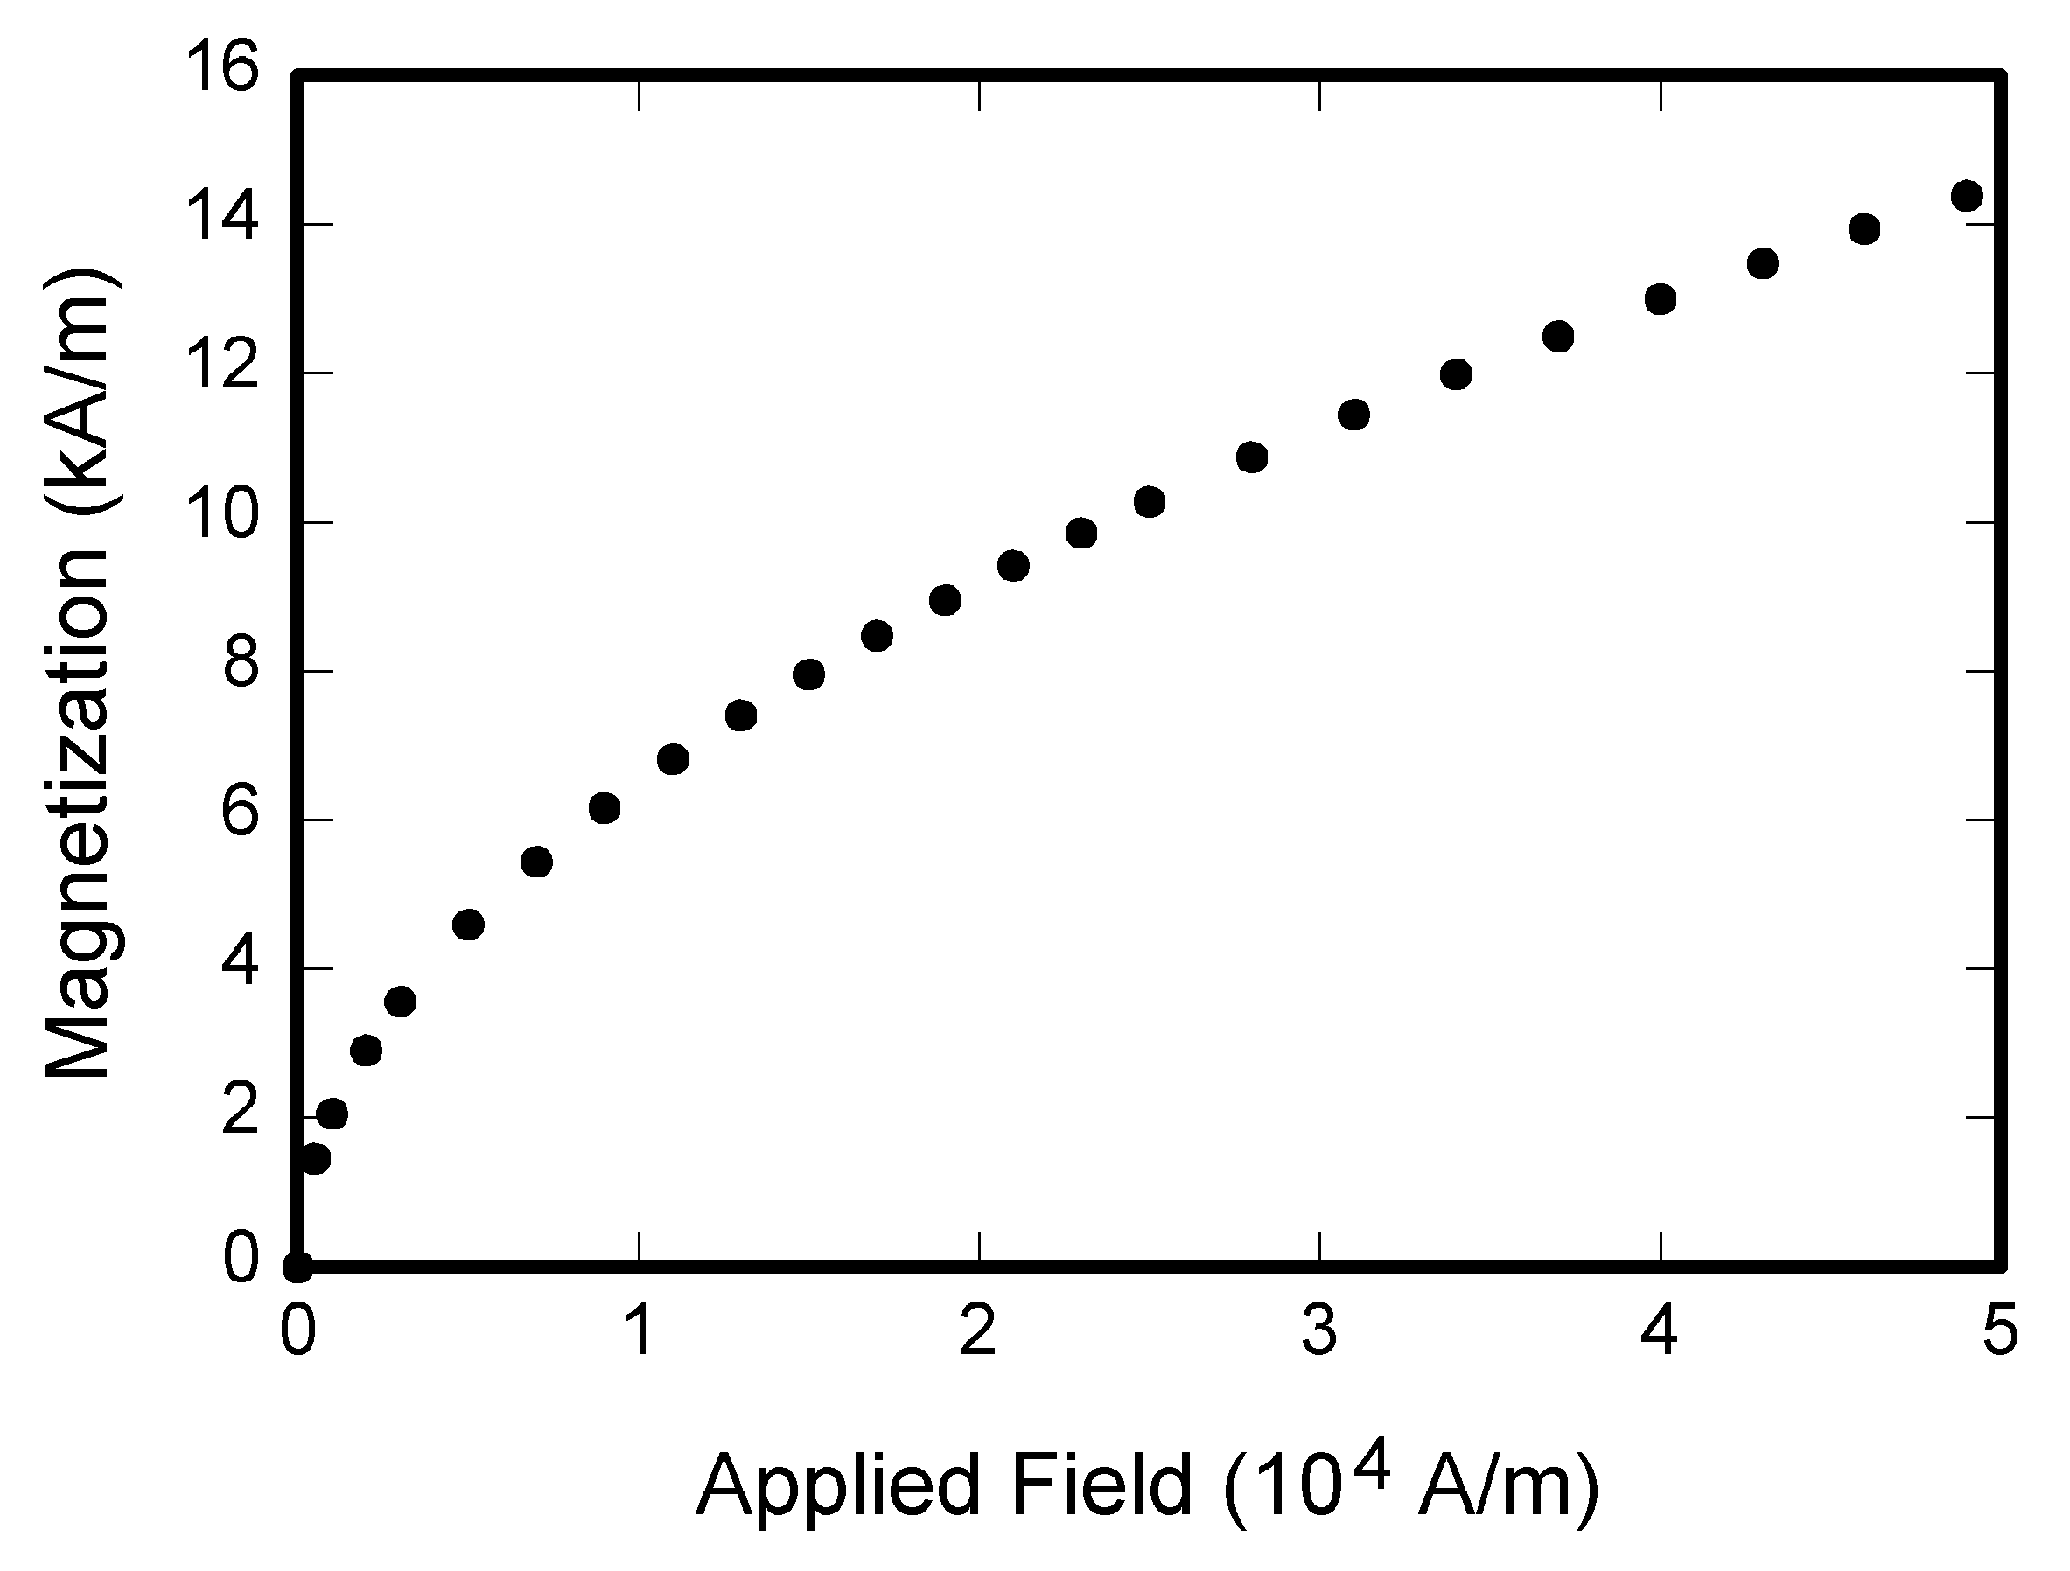
\includegraphics[width=18.5pc]{fig/fig1.png}}
\caption{regional split of basins}
\end{figure}

Decomposition:
	1. Relative power of EOFs in spatial decomposition + Sample maps of EOFs (how many?)
	2. Projection co-efficient PSDs? (to showcase most dominant temporal modes) 
5. Generator:
	1. Phase randomized projection co-efficients for ensemble of realizations
	2. Generated realizations - Power Spectral Densities comparison (specific basins of interest? Amery, Filchner-Ronne, Ross/Thwaites)
\section{DISCUSSION}
This forcing can be used in ice sheet models to study the impact of internal climate variability on the ice sheet and its response to changing climate conditions.

\section{CONCLUSION}
The manuscript should include a conclusion. In this section, summarize what was described in your paper. Future directions may also be included in this section. Authors are strongly encouraged not to reference multiple figures or tables in the conclusion; these should be referenced in the body of the paper. Looking forward statements. This technique can be used as a flexible source of ensemble members for future climate and ice sheet projections. We show that the projections of the basal melt arising from the generated alternate forcings are statistically consistent with those from the E3SM simulation in terms of the large-scale spatial variability. We also find that the method captures the variability in the timing of (peak?) melt rates. This generator can be applied to any large-scale ice sheet model that is forced by a global climate model and help to reduce the computational cost of generating large ensemble simulations of the AIS under historical and future forcing scenarios to better quantify SLR uncertainty arising from the AIS.
\section{APPENDIX}
Nothing yet.
\section{ACKNOWLEDGMENT}
This work was supported in part by the U.S. National Science Foundation under Award 1947882, as part of the Antarctic Ice Sheet Large Ensemble (AISLENS) project.
\begin{thebibliography}{1}

\bibitem{adusimilli2020}
Adusumilli, S., Fricker, H.A., Medley, B. et al. Interannual variations in meltwater input to the Southern Ocean from Antarctic ice shelves. Nat. Geosci. 13, 616–620 (2020). https://doi.org/10.1038/s41561-020-0616-z

\bibitem{comeau2022}
Comeau, D., Asay-Davis, X. S., Begeman, C. B., Hoffman, M. J., Lin, W., Petersen, M. R., et al. (2022). The DOE E3SM v1.2 cryosphere configuration: Description and simulated Antarctic ice-shelf basal melting. Journal of Advances in Modeling Earth Systems, 14, e2021MS002468. https://doi.org/10.1029/2021MS002468

\bibitem{link2019}
Link, R., Snyder, A., Lynch, C., Hartin, C., Kravitz, B., and Bond-Lamberty, B.: Fldgen v1.0: an emulator with internal variability and space–time correlation for Earth system models, Geosci. Model Dev., 12, 1477–1489, https://doi.org/10.5194/gmd-12-1477-2019, 2019.

\end{thebibliography}
\begin{IEEEbiography}{S. Muruganandham}{\,}is with Georgia Tech, Atlanta, U.S.A.. Mr. Muruganandham's biography appears here.  Contact him/her at faauthor@xyz.com.
\end{IEEEbiography}

\begin{IEEEbiography}{A.A. Robel,}{\,}is with Georgia Tech, Atlanta, U.S.A.. Dr. Robel's biography appears here.  Contact him/her at sbauthor@abc.com.
\end{IEEEbiography}

\begin{IEEEbiography}{M. Hoffman}{\,}is with LANL, New Mexico, U.S.A. Dr. Hoffman's biography appears here.  Contact him/her at tcauthor@def.com.
\end{IEEEbiography}

\begin{IEEEbiography}{S. Price}{\,}is with LANL, New Mexico, U.S.A. Dr. Price's biography appears here.  Contact him/her at tcauthor@def.com.
\end{IEEEbiography}

\end{document}